\subsection{Experiment 1 and 2: Correlation Analysis and Importance Analysis}

In the experiment 1, the correlation analysis workflow computed the Pearson correlation matrix over the features in the \texttt{PWDriverFeatureSet} dataset. In the experiment 2, it first removed outliers using an isolation forest fitted to the joint predictor-target space, and then trained a random forest regressor on the filtered data.

\begin{figure}[H]
	\centering
	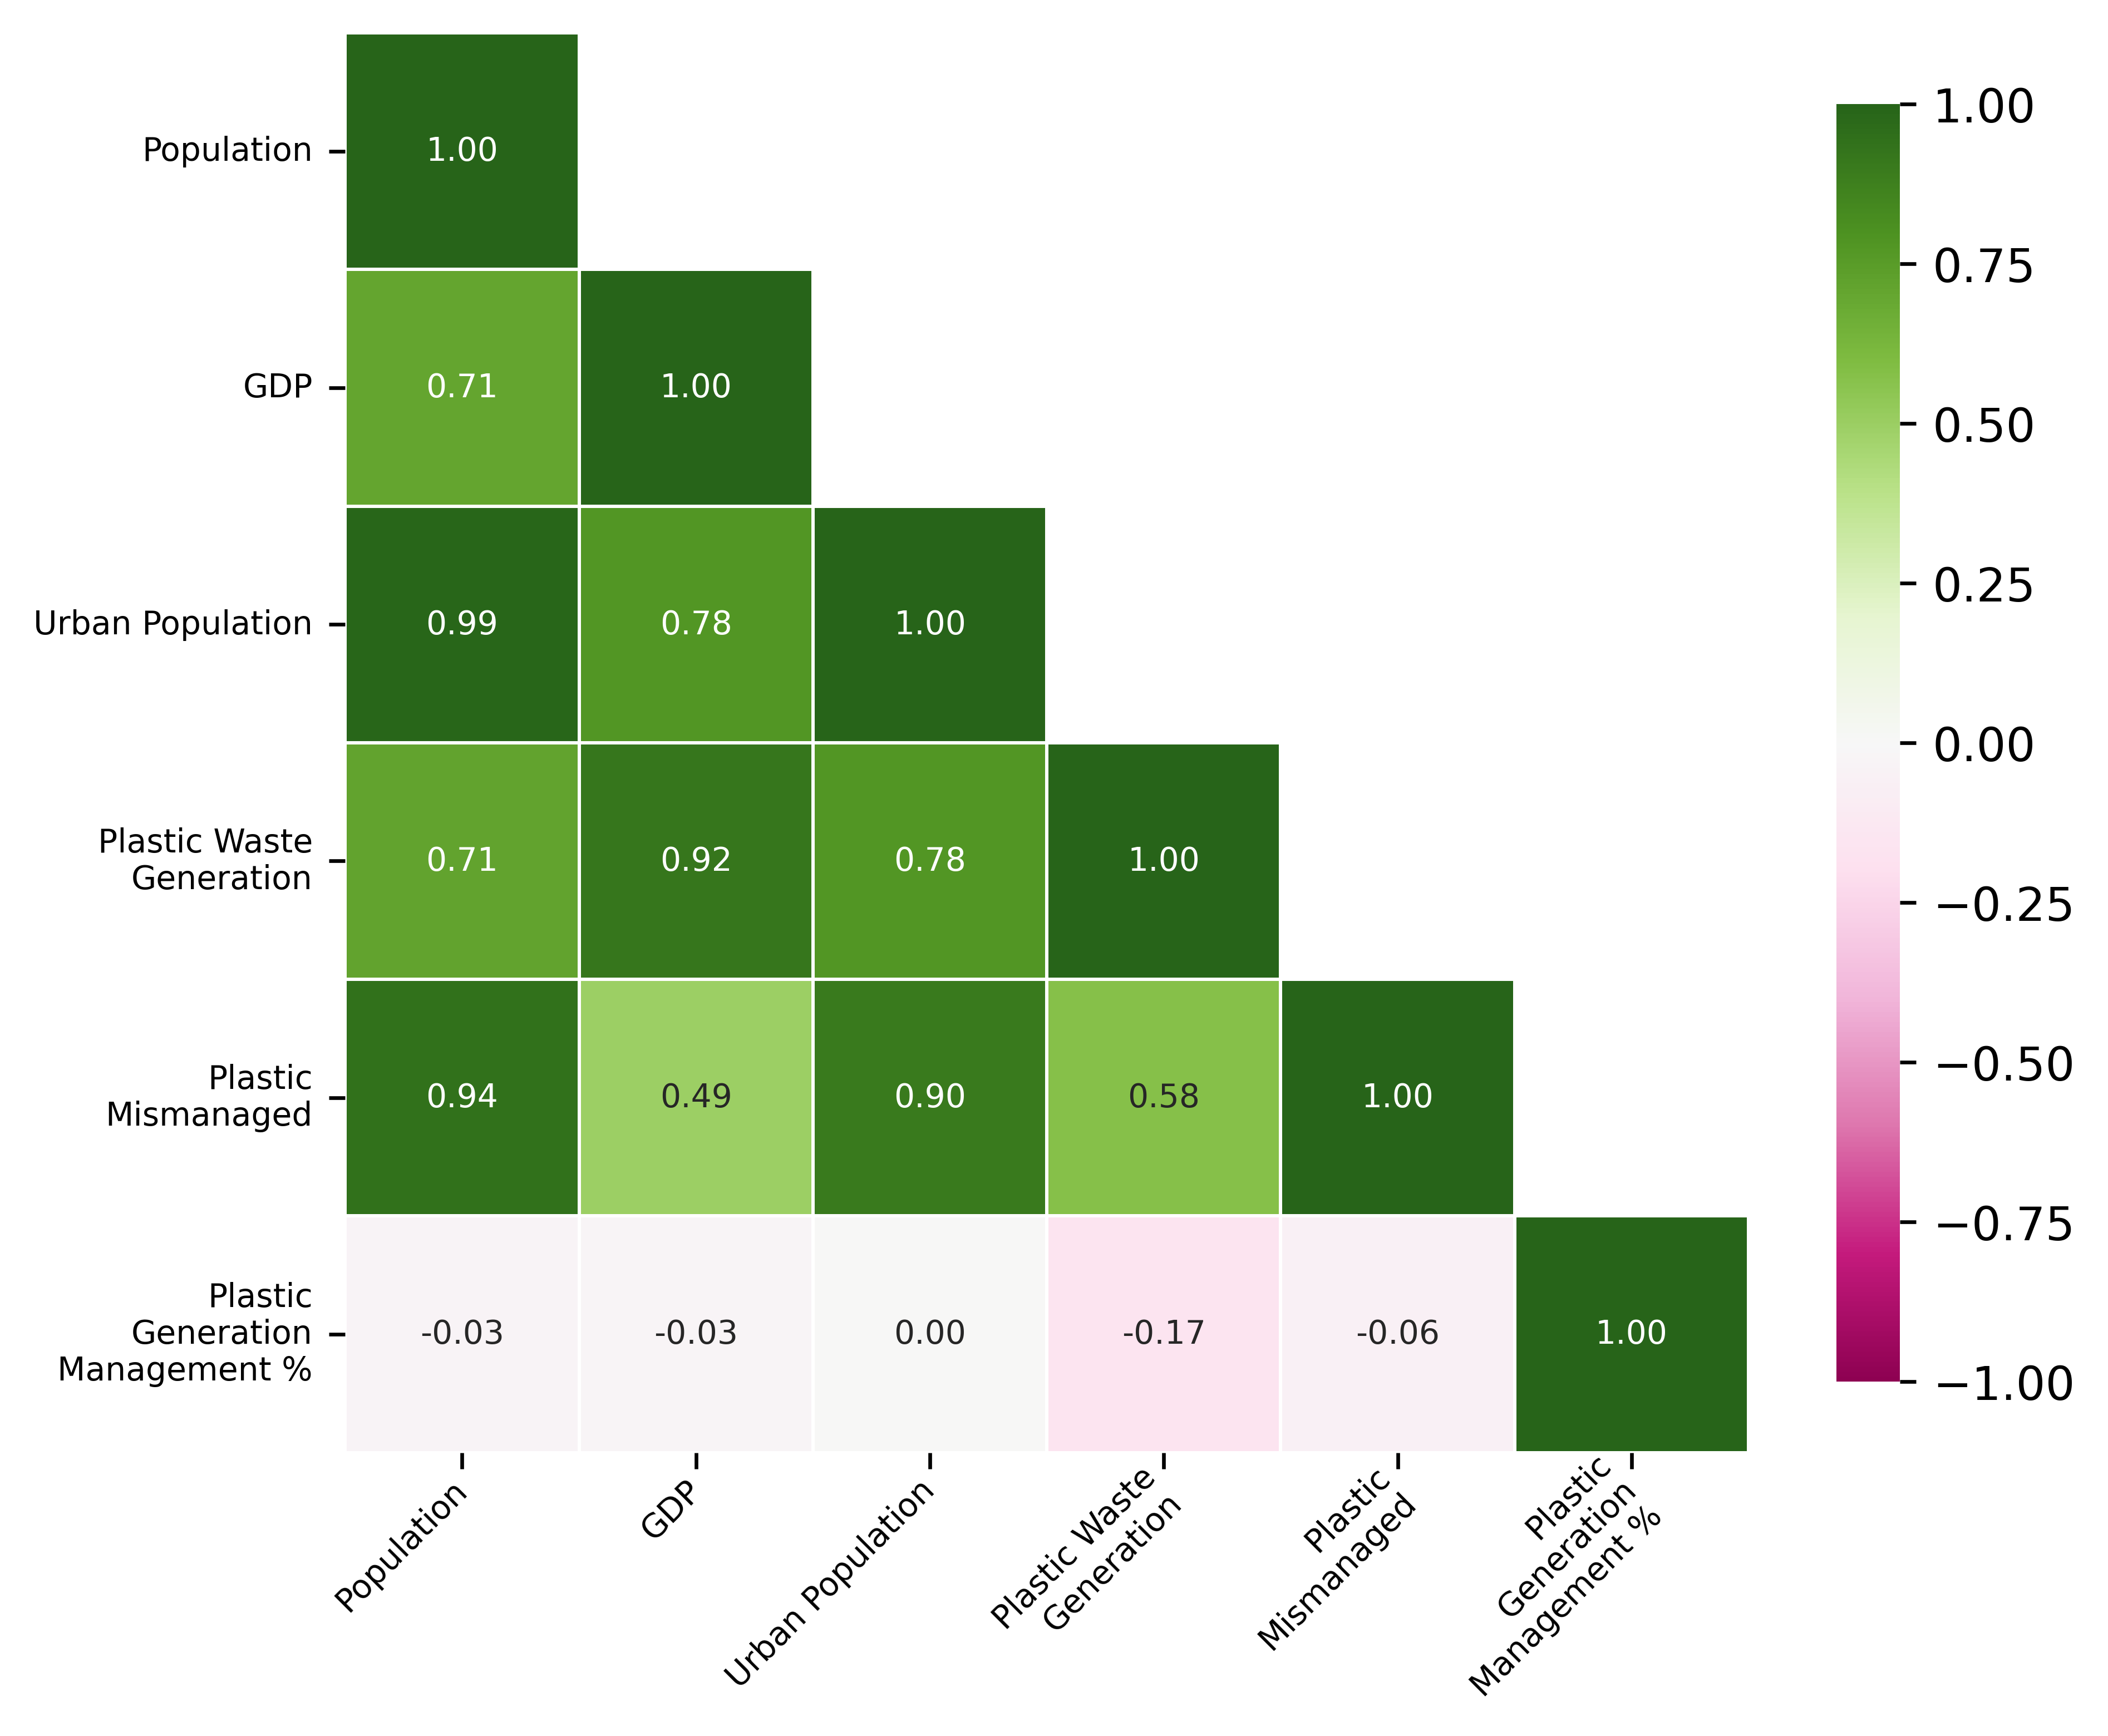
\includegraphics[width=0.8\linewidth]{figures/correlation_matrix.png}
	\caption{
		\centering
		Correlation matrix for the pooled \texttt{PWDriverFeatureSet} dataset. It summarizes pairwise association patterns across the pooled driver set.
	}
	\label{fig:correlation_matrix}
\end{figure}

Figure~\ref{fig:correlation_matrix} shows that GDP is strongly associated with plastic waste generation (\(r = 0.92\)). The correlation between urban population and plastic waste generation (\(r = 0.78\)) is stronger than that of total population (\(r = 0.71\)). Population and mismanaged plastic waste are also highly correlated (\(r = 0.94\)). In contrast, the percentage of plastic waste that is properly managed is nearly orthogonal to the scale variables and exhibits a weak negative correlation with plastic waste generation (\(r = -0.166\)).

\begin{figure}[H]
	\centering
	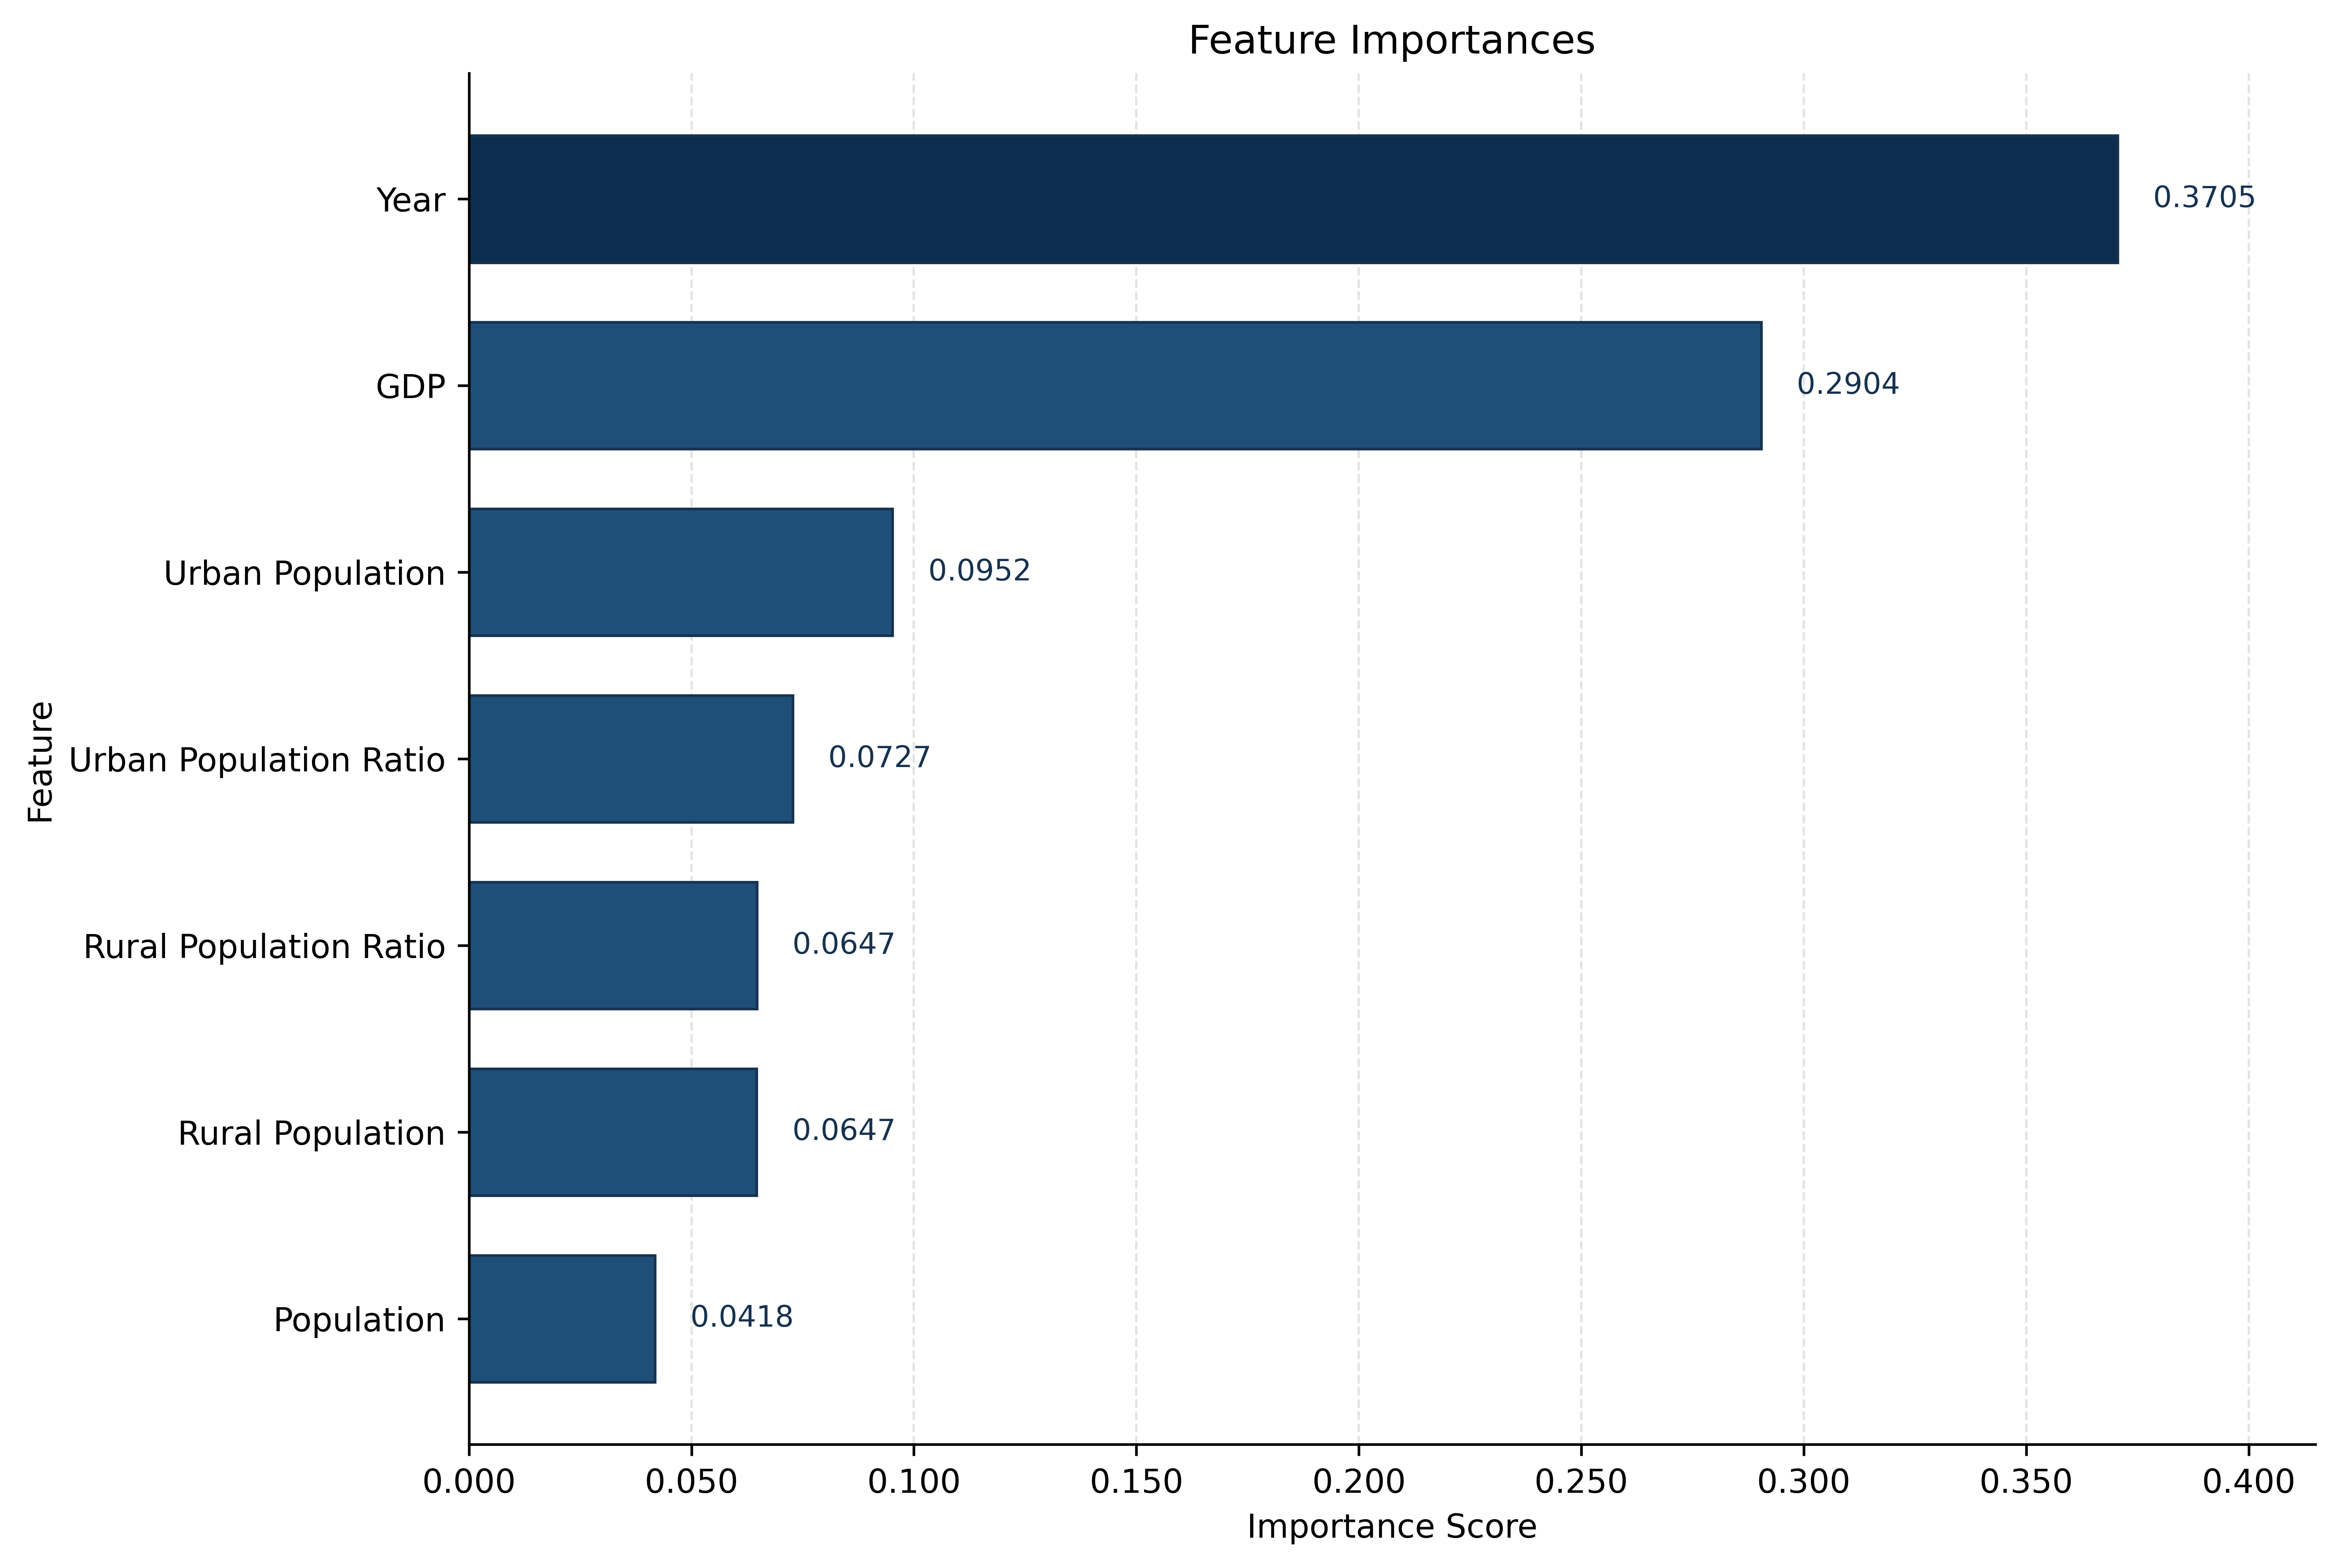
\includegraphics[width=1.0\linewidth]{figures/feature_importances.png}
	\caption{
		\centering
		Feature importances for the \texttt{PWGPredictors} dataset. This histogram shows the relative importance of each feature in predicting plastic waste generation.
	}
	\label{fig:feature_importances}
\end{figure}

Experiment~2 extends the correlation analysis by incorporating target-aware ranking. Figure~\ref{fig:feature_importances} indicates that \textit{year} has the highest importance score (0.3764), followed by GDP (0.2582). The importance of urban population (0.0821) is slightly greater than that of rural population (0.0690) and total population (0.0442). This finding is consistent with recent work, which shows that urban areas contribute disproportionately to plastic waste generation due to higher consumption of single-use plastics and packaged goods~\cite{sen2026unveiling}.

